\documentclass{scrartcl}
\usepackage[a4paper,margin=2cm,footskip=1cm]{geometry}
\setkomafont{disposition}{\normalfont\bfseries}

%\documentclass{article}

\usepackage[table,xcdraw]{xcolor}
\usepackage{tikz}
\usetikzlibrary{angles,quotes}
\usetikzlibrary{babel}

\usepackage{booktabs}
\usepackage[utf8]{inputenc}
\usepackage[spanish, es-nodecimaldot]{babel}
\usepackage[per-mode=symbol]{siunitx}
\usepackage{graphicx}
\usepackage{subcaption}
\usepackage{caption}
\usepackage{mathtools}
\usepackage{amsmath}
\usepackage{slashed}
\usepackage{dsfont}
\usepackage{float}
\usepackage{multicol}
\usepackage{wrapfig}
\usepackage{lipsum}
\usepackage{textcomp}
\usepackage{gensymb}
\usepackage{longtable}
\usepackage{supertabular}
\usepackage{hhline}
\usepackage{enumerate}
\usepackage{multirow}
\usepackage{amssymb}
\usepackage{tabularx}
\usepackage{ragged2e}
\usepackage{rotating}
\usepackage{cancel}
\usepackage{physics}
\usepackage[framemethod=default]{mdframed}
\usepackage{csquotes}
%\usepackage[backend=biber, style=numeric, sorting=none]{biblatex}
\usepackage{qcircuit}
\usepackage{bm}

\renewcommand{\figurename}{Figura}
\renewcommand{\spanishtablename}{Tabla}
\newcommand{\inv}[1]{\frac{1}{#1}}
\newcommand{\uv}[1]{\hat{\mathbf{#1}}}
\newcommand{\uvs}[1]{\, \uv{#1}}

\newcommand{\realSet}{\mathbb{R}}
\newcommand{\complexSet}{\mathbb{C}}
\newcommand{\oref}{$\mathcal{O}$ }
\newcommand{\opref}{$\mathcal{O}'$ }
\newcommand{\oppref}{$\mathcal{O}''$ }

\def\residue{\mathop{\text{Res}}}

\setlength{\tabcolsep}{19pt}

\DeclareSIUnit\clight{\text{\ensuremath{c}}}
\DeclareSIUnit\MeV{\mega\electronvolt}
\DeclareSIUnit\GeV{\giga\electronvolt}
\DeclareSIUnit\MeVpc{\MeV\per\clight\squared}
\DeclareSIUnit\GeVpc{\GeV\per\clight\squared}

%\newcommand{\vbeta}{\vb{\beta}}
\newcommand{\sinc}{\text{sinc}}
\newcommand{\E}{\vb{E}}
\newcommand{\B}{\vb{B}}
\newcommand{\x}{\vb{x}}
\newcommand{\y}{\vb{y}}
\newcommand{\z}{\vb{z}}
\newcommand{\p}{\vb{p}}
\renewcommand{\k}{\vb{k}}
\newcommand{\Lag}{\mathcal{L}}
\newcommand{\Ham}{\mathcal{H}}

\newcommand{\tx}{\tilde{x}}

\renewcommand{\vb}[1]{\bm{#1}}

\renewcommand{\a}[1]{\hat{a}_{#1}}
\newcommand{\ad}[1]{\hat{a}_{#1}^\dagger}

\DeclareRobustCommand{\[}{\begin{equation}}
\DeclareRobustCommand{\]}{\end{equation}}
\mathtoolsset{showonlyrefs}

\allowdisplaybreaks

%\bibliography{bibliography}

%----------------------------------------------------------------------------------------
%	DOCUMENT INFORMATION
%----------------------------------------------------------------------------------------

\title{Teoría de la Información Cuántica}
\subtitle{Práctica 3 - Año 2020}
\author{\textsc{Beaucamp}, Jean Yves}
\date{}

\begin{document}

\maketitle

\section{Compuertas Lógicas Cuánticas}
\begin{enumerate}
    
    %-------------------------------------------------------------------------------------------------------
    %   Problema I.1
    %-------------------------------------------------------------------------------------------------------
    \item Sabemos que podemos escribir el operador densidad de un qubit como una matriz $\rho \in \complexSet^{2x2}$ dada por $\rho = \inv{2} (\mathds{1} + \vb{r} \vdot \vb{\sigma})$. Por lo tanto, buscamos una expresión de los operadores de rotación en la representación de $\complexSet^{2x2}$. Sabemos que $\{ \sigma_x, \sigma_y, \sigma_z \}$ son una base del álgebra de generadores de $su(2)$. Por lo tanto, $e^{-i\sigma_k}$, para $k = x, y, z$, será una base del grupo de matrices unitarias de determinante 1, es decir, si $M \in SU(2)$, entonces $M = R_{\vu{n}}(\theta) = e^{-i\theta \vu{n} \vdot \vb{\sigma}/2}$ para algún $\theta \in \realSet$ y $\vu{n}$ vector unitario. Para pasar de $SU(2)$ a $U(2)$ solo deberemos multiplicar $M$ por una fase compleja arbitraria, ya que
    \[ \det(e^{i\alpha} M) = e^{i2\alpha} \det{M} = e^{i2\alpha}. \]
    Por lo tanto, toda transformación unitaria de un qubit (matrices unitarias de 2x2) podrá ser escrita como
    \[ U = e^{i\alpha} R_{\vu{n}}(\theta) = e^{-i\theta \vu{n} \vdot \vb{\sigma}/2}. \]
    
    
    
    %-------------------------------------------------------------------------------------------------------
    %   Problema I.2
    %-------------------------------------------------------------------------------------------------------
    \item Para el caso general, como $(\vu{n} \vdot \vb{\sigma})^2 = \mathds{1}$ (ya que $\sigma_k^2 = \mathds{1}$), y por consiguiente $(\vu{n} \vdot \vb{\sigma})^{2n} = 1$ y $(\vu{n} \vdot \vb{\sigma})^{2n+1} = \vu{n} \vdot \vb{\sigma}$, las matrices de rotación de qubits $R_{\vu{n}}(\theta)$ podrán ser expresadas como
    \begin{align}
        R_{\vu{n}}(\theta) = \sum_{k = 0}^\infty \frac{(-i\theta/2)^{2k}}{(2k)!} \mathds{1} + \sum_{k = 0}^\infty \frac{(-i\theta/2)^{2k+1}}{(2k+1)!} \vu{n} \vdot \vb{\sigma} &= \mathds{1} \cosh(\frac{i\theta}{2}) + \vu{n} \vdot \vb{\sigma} \sinh(\frac{-i\theta}{2}) \\
            &= \mathds{1} \cos(\frac{\theta}{2}) - i \vu{n} \vdot \vb{\sigma} \sin(\frac{\theta}{2}).
    \end{align}
    
    Por lo tanto,
    \[ i R_x(\pi) = i \qty( \mathds{1} \cancel{\cos(\frac{\pi}{2})} - i \vu{x} \vdot \vb{\sigma} \sin(\frac{\pi}{2}) ) = -i^2 \sigma_x = \sigma_x = X, \]
    \[ i R_y(\pi) = i \qty( \mathds{1} \cancel{\cos(\frac{\pi}{2})} - i \vu{y} \vdot \vb{\sigma} \sin(\frac{\pi}{2}) ) = -i^2 \sigma_y = \sigma_y = Y, \]
    y
    \[ i R_z(\pi) = i \qty( \mathds{1} \cancel{\cos(\frac{\pi}{2})} - i \vu{z} \vdot \vb{\sigma} \sin(\frac{\pi}{2}) ) = -i^2 \sigma_z = \sigma_z = Z. \]
    
    Para el caso de la compuerta Hadamard, si $\vu{n} = \inv{\sqrt{2}}(1, 0, 1)$, entonces
    \[
        i R_{\vu{n}}(\pi) = i \qty( \mathds{1} \cancel{\cos(\frac{\pi}{2})} - i \inv{\sqrt{2}} (1, 0, 1) \vdot \vb{\sigma} \sin(\frac{\pi}{2}) ) = \inv{\sqrt{2}} (\sigma_x + \sigma_z) = \inv{\sqrt{2}}
        \begin{pmatrix} 1 & 1 \\ 1 & -1 \end{pmatrix}
        = H.
    \]
    
    Finalmente, como $\sigma_k^\dagger = \sigma_k$, y $H^\dagger = H$, entonces analizándolo en términos geométricos, $X Z X = X Z X^\dagger = R_x(\pi) Z R_x(-\pi) = -Z$, pudiendo ser interpretado como una rotación en $\pi$ sobre el eje $x$, invirtiendo la orientación de un vector inicial en la dirección $z$ a $-z$. Bajo la misma justificación geométrica, $X Y X = X Y X^\dagger = R_x(\pi) Y R_x(-\pi) = -Y$. Con un razonamiento análogo, como podemos ver en la fig. \ref{fig:I_2}, $H X H = R_{\vu{n}}(\pi) X R_{\vu{n}}(\pi) = Z$. Como además $H$ es autoadjunto, entonces también se cumple $H Z H = X$ (gráficamente evidente).
    \begin{figure}[t]
        \centering
        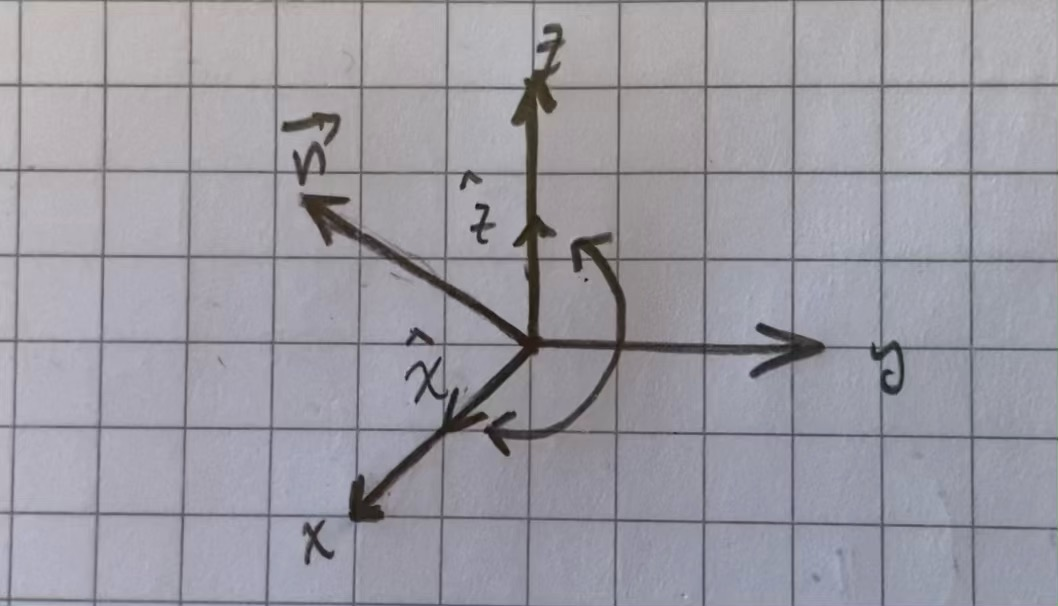
\includegraphics[width=.4\linewidth]{Images/IMG_3078.JPEG}
        \caption{Rotación en $\pi$ alrededor del eje $\vu{n} = \inv{\sqrt{2}} (1, 0, 1)$ de un vector unitario $\vu{x}$ a $\vu{z}$.}
        \label{fig:I_2}
    \end{figure}
    
    
    
    %-------------------------------------------------------------------------------------------------------
    %   Problema I.3
    %-------------------------------------------------------------------------------------------------------
    \item Buscamos un tiempo $t$ y un Hamiltoniano $H$ de dos qubits tal que el operador de evolución unitaria $U(t)$ cumpla
    \[ U(t) = \exp{\frac{-iHt}{\hbar}} \equiv R_{\vu{n}}(\theta) \otimes R_{\vu{m}}(\phi). \]
    Es fácil ver que $e^{\mathds{1} \otimes A} = \mathds{1} \otimes e^A$:
    \[ e^{\mathds{1} \otimes A} = \sum_{n = 0}^\infty \frac{(\mathds{1} \otimes A)^n}{n!} = \sum_{n = 0}^\infty \frac{\mathds{1} \otimes A^n}{n!} = \mathds{1} \otimes \left( \sum_{n = 0}^\infty \frac{A^n}{n!} \right) = \mathds{1} \otimes e^A. \]
    De forma análoga se puede demostrar que $e^{A \otimes \mathds{1}} = e^A \otimes \mathds{1}$. Por lo tanto, el problema se reduce a obtener $e^M = R_{\vu{n}}(\theta)$ y $e^N = R_{\vu{m}}(\phi)$, y expresarlo en la forma de un operador de evolución temporal. Por lo estudiado en II.1, sabemos que $R_{\vu{n}}(\theta) = e^{-i \frac{\theta}{2} \vu{n} \vdot \vb{\sigma}}$. Utilizando la definición del operador de Spin $\vb{S} = \frac{\hbar}{2} \vb{\sigma}$, entonces:
    \[ R_{\vu{n}}(\theta) = e^{-i \frac{\theta}{2} \vu{n} \vdot \vb{\sigma}} = e^{-i \theta \vu{n} \vdot \frac{\vb{S}}{\hbar}} = e^{\frac{-i H_{\theta \vu{n}} t}{\hbar}}, \]
    con $H_{\theta \vu{n}} = \theta \vu{n} \vdot \vb{S} = \frac{\hbar}{2} \vu{n} \vdot \vb{\sigma}$, que corresponde al hamiltoniano de Spin para un electrón inmerso en un campo magnético $\vb{B} = \theta \vu{n}$. El tiempo, en este caso, corresponderá a $t = 1$. Para $R_{\vu{m}}(\phi)$ el resultado es equivalente, obteniendo $H_{\phi \vu{m}} = \phi \vu{m} \vdot \vb{S} = \frac{\hbar}{2} \vu{n} \vdot \vb{\sigma}$. Por lo tanto,
    \[ H = H_{\theta\vu{n}} \otimes \mathds{1} + \mathds{1} \otimes H_{\phi\vu{m}} = \frac{\hbar}{2} \theta \vu{n} \vdot \vb{\sigma} \otimes \mathds{1} + \mathds{1} \otimes \frac{\hbar}{2} \phi \vu{m} \vdot \vb{\sigma}, \quad \quad t = 1. \]
    Si se desea realizar la operación en un tiempo $t = t_0$, basta solo con escalar los campos magnéticos $\vb{B}_A = \theta \vu{n} \to \frac{\theta}{t_0} \vu{n}$ y $\vb{B}_B = \phi \vu{m} \to \frac{\phi}{t_0} \vu{m}$.
    
    
    \item Resulta útil primero realizar un cambio de base para obtener un operador de interacción diagonal. Por lo demostrado en I.2, sabemos que $H Z H = X$. Entonces,
    \[
        \begin{array}{c}
            \Qcircuit @C=1.4em @R=1.2em {
                & \ctrl{1}  & \qw \\
                & \targ     & \qw
            }
        \end{array}
        \quad \quad
        =
        \begin{array}{c}
            \Qcircuit @C=1.4em @R=1.2em {
                & \ctrl{1} & \qw \\
                & \gate{X} & \qw
            }
        \end{array}
        \quad \quad
        =
        \quad \quad
        \begin{array}{c}
            \Qcircuit @C=1.4em @R=1.2em {
                & \qw       & \ctrl{1}  & \qw       & \qw \\
                & \gate{H}  & \gate{Z}  & \gate{H}  & \qw
            }
        \end{array}
        \quad .
    \]
    Entonces, el problema de ahora se reduce a obtener un hamiltoniano compatible con un operador de interacción diagonal
    \[ U_{CZ} = \dyad{0}{0} \otimes \mathds{1} + \dyad{1}{1} \otimes Z \equiv \begin{pmatrix} \mqty{\dmat{1,1,1,-1}} \end{pmatrix}. \label{eq:I4_1} \]
    Por su carácter diagonal, es intuitivo construir $H$ como
    \[ H = \alpha \sigma_z \times \mathds{1} + \beta \mathds{1} \otimes \sigma_z + \gamma \sigma_z \otimes \sigma_z + \nu \mathds{1} \otimes \mathds{1}. \]
    Podemos despreciar el término en $\mathds{1} \otimes \mathds{1}$ al representar únicamente una fase global. Además, para que sea simétrico, $\alpha = \beta$, y $\gamma = \alpha \xi$. Luego,
    \[ H = \alpha (\sigma_z \otimes \mathds{1} + \mathds{1} \otimes \sigma_z + \xi \sigma_z \otimes \sigma_z ), \]
    obteniendo en cada estado
    \[
        \begin{array}{ll}
            H \ket{00} = \alpha (2 + \xi) \ket{00}, & H \ket{10} \alpha (-1 + 1 - \xi) \ket{10} = -\alpha\xi \ket{10 }, \\
            H \ket{01} = \alpha (1 - 1 - \xi) \ket{01} = -\alpha \xi \ket{01}, & H \ket{11} = (-1 - 1 + \xi (-1)^2 ) \ket{11} = -\alpha (2 - \xi) \ket{11}.
        \end{array}
    \]
    Para que el resultado resulte idéntico en $\ket{00}$, $\ket{01}$ y $\ket{10}$ (compatible con \eqref{eq:I4_1}), vemos que $\xi = -1$, por lo que entonces el hamiltoniano se reduce a
    \[ H = \alpha (\sigma_z \otimes \mathds{1} + \mathds{1} \otimes \sigma_z - \sigma_z \otimes \sigma_z ) = \alpha \begin{pmatrix} \mqty{\dmat{1, 1, 1, -3}} \end{pmatrix}. \]
    Por lo tanto,
    \begin{align}
        U_{CZ} = e^{\frac{-iHt}{\hbar}} = \exp{-i\omega t \begin{pmatrix} \mqty{\dmat{1, 1, 1, -3}} \end{pmatrix}} &=
        \begin{pmatrix}
            \mqty{\dmat{e^{-i\omega t}, e^{-i\omega t}, e^{-i\omega t}, e^{3i\omega t}}}
        \end{pmatrix} \\
        &= e^{-i\omega t}
        \begin{pmatrix}
            \mqty{\dmat{1, 1, 1, e^{4i\omega t}}}
        \end{pmatrix}
    \end{align}
    donde se ha definido $\omega = \alpha / \hbar$. Buscar que el último elemento de la diagonal sea $-1$ (para obtener \eqref{eq:I4_1}) nos impone una condición sobre $t$ y $\omega$ como
    \[ 4\omega t = \pi + 2n\pi \implies t = \frac{(1+2n)}{4\omega} \pi. \]
    El factor exponencial remanente resulta una fase global, por lo que no es relevante en la medición final del sistema.
    
    La compuerta $U_{CNOT}$ podrá ser entonces realizada por
    \[ U_{CX} = (\mathds{1} \otimes H_{ad} ) U_Z (\mathds{1} \otimes H_{ad}), \]
    donde $H_{ad}$ es el operador de la compuerta Hadamard, con hamiltoniano 
    \[ H_{Had} = \mathds{1} \otimes \frac{\hbar \pi}{2 \sqrt{2}} (\sigma_x + \sigma_z). \]
    
\end{enumerate}


\section{Estados de dos qubits y traspuesta parcial.}
\begin{enumerate}
    
    %-------------------------------------------------------------------------------------------------------
    %   Problema II.1
    %-------------------------------------------------------------------------------------------------------
    \item Podemos describir de forma general un estado de dos qubits por medio de su matriz densidad, expresada como
    \[ \rho_{AB} = \inv{4} \left[ \mathds{1} \otimes \mathds{1} + \vb{r}_A \vdot \vb{\sigma} \otimes \mathds{1} + \mathds{1} \otimes \vb{\sigma} \vdot \vb{r}_B + \sum_{i, j = 1}^3 J_{ij} \sigma_i \otimes \sigma_j \right]. \label{eq:II_1_def} \]
    
    \begin{enumerate}
        \item Como
        \[ \Tr{(\sigma_i \otimes \sigma_j)(\sigma_{i'} \otimes \sigma_{j'})} = \Tr_A (\sigma_i \sigma_{i'}) \Tr_B (\sigma_j \sigma_{j'}) = 2 \delta_{i i'} \ 2 \delta_{j j'} = 4 \delta_{i i'} \delta_{j j'}, \]
        entonces es trivial ver que
        \[ \expval{\vb{\sigma}_A} = \Tr(\rho_{AB} \vb{\sigma} \otimes \mathds{1}) = \vb{r}_A, \]
        \[ \expval{\vb{\sigma}_B} = \Tr(\rho_{AB} \mathds{1} \otimes \vb{\sigma}) = \vb{r}_B, \]
        y
        \[ \expval{\sigma_i \otimes \sigma_j} = \Tr(\rho_{AB} \sigma_i \otimes \sigma_j) = J_{ij}. \]
        
        
        \item La matriz densidad del sistema puede ser escrita de manera más compacta como
        \[ \rho = \sum_{\mu\nu}^4 J_{\mu\nu} \sigma_\mu \otimes \sigma_\nu. \]
        No necesariamente la matriz $J_{\mu\nu}$ del sistema resulta diagonal, por lo que no está garantizado que pueda ser diagonalizada. Sin embargo, como si admite una descomposición en valores singulares, los ejes locales de los subsistemas $A$ y $B$ si pueden ser rotados individualmente (recordamos que toda matriz unitaria, en particular las matrices $V$ y $W$ de cambio de base en la SVD, pueden ser expresadas como rotaciones generales como se ha demostrado en el ejercicio I.1) tal que el sistema resultante si adquiera una forma
        \[ \rho'_{AB} = \sum_{\nu = 1}^{n_s} \lambda_\nu \sigma'_\nu \otimes \sigma''_\nu. \]
        
        
        \item Las matrices densidad reducidas $\rho_A$ y $\rho_B$ estarán determinadas por los elementos de matriz
        \[ \mel{0}{\sigma_x}{0} = \mel{1}{\sigma_x}{1} = \mel{0}{\sigma_y}{0} = \mel{1}{\sigma_y}{1} = 0, \quad \quad \mel{0}{\sigma_z}{0} = 1, \quad \quad \mel{1}{\sigma_z}{1} = -1. \]
        Luego,
        \begin{align}
            \rho_B &= \Tr_A \rho_{AB} \\
                &= \inv{4} \left( 2 \mathds{1}_B + r^A_z (\cancel{\mel{0}{\sigma_z^A}{0} + \mel{1}{\sigma_z^A}{1}}) \mathds{1}_B + 2 \vb{\sigma}_B \vdot \vb{r}_B \right. \\
                &\quad \quad \left. + \sum_{i = 1}^3 (\cancel{\mel{0}{\sigma_z^A}{0} + \mel{1}{\sigma_z^A}{1}}) \sum_{j = 1}^3 J_{3j} \sigma^B_j \right) \\
                &= \inv{4} \left( 2 \mathds{1}_B + 2 \vb{\sigma}_B \vdot \vb{r}_B \right) \\
                &= \inv{2} \left( \mathds{1}_B + \vb{\sigma}_B \vdot \vb{r}_B \right).
        \end{align}
        
        Por un procedimiento análogo podemos encontrar la matriz densidad reducida $\rho_A$, obteniendo
        \[ \rho_A = \Tr_B \rho_{AB} = \inv{2} \left( \mathds{1}_A + \vb{\sigma}_A \vdot \vb{r}_A \right). \]
        
        
        \item La matriz traspuesta parcial respecto a $B$ de $\rho_{AB}$ estará determinada por
        \[ \sigma_x^t = \sigma_x, \quad \sigma_y^t = -\sigma_y, \quad \sigma_z^t = \sigma_z. \]
        Luego,
        \begin{align}
            \rho_{AB}^{t_B} &= \inv{4} \left[ \mathds{1} \otimes \mathds{1}^t + \vb{r}_A \vdot \vb{\sigma} \otimes \mathds{1}^t + \mathds{1} \otimes \vb{\sigma}^t \vdot \vb{r}_B + \sum_{i, j = 1}^3 J_{ij} \sigma_i \otimes \sigma_j^t \right] \\
                &= \inv{4} \left[ \mathds{1} \otimes \mathds{1} + \vb{r}_A \vdot \vb{\sigma} \otimes \mathds{1} + \mathds{1} \otimes \vb{\sigma} \vdot (r_x^B, -r_y^B, r_z^B) + \sum_{i, j = 1}^3 J_{ij} \sigma_i \otimes \sigma_j^t \right].
        \end{align}
        
        
        \item Utilizando el Mathematica y las expresiones para $\vb{r}_A$, $\vb{r}_B$ y $\vb{J}_{ij}$ encontradas en II.1.a, podemos encontrar la forma \eqref{eq:II_1_def} de los siguientes estados puros:
        \begin{enumerate}[(i)]
            \item $\ket{\Psi} = \inv{\sqrt{2}} (\ket{00} + \ket{11})$.
            \[
                \rho_{AB} = \dyad{\Psi}{\Psi} = \inv{2}
                \begin{pmatrix}
                    1 & 0 & 0 & 1 \\
                    0 & 0 & 0 & 0 \\
                    0 & 0 & 0 & 0 \\
                    1 & 0 & 0 & 1
                \end{pmatrix}.
            \]
            
            Luego,
            \[ \vb{r}_A = \Tr(\rho_{AB} \vb{\sigma} \otimes \mathds{1}) = (0, 0, 0), \]
            \[ \vb{r}_B = \Tr(\rho_{AB} \mathds{1} \otimes \vb{\sigma}) = (0, 0, 0), \]
            y
            \[
                J_{ij} = \Tr(\rho_{AB} \sigma_i \otimes \sigma_j) =
                \begin{pmatrix}
                    1 & 0 & 0 \\
                    0 & -1 & 0 \\
                    0 & 0 & 1 \\
                \end{pmatrix}.
            \]
            
            
            \item $\ket{\Psi} = \inv{\sqrt{2}} (\ket{01} - \ket{10})$.
            \[
                \rho_{AB} = \dyad{\Psi}{\Psi} = \inv{2}
                \begin{pmatrix}
                    0 & 0 & 0 & 0 \\
                    0 & 1 & -1 & 0 \\
                    0 & -1 & 1 & 0 \\
                    0 & 0 & 0 & 0
                \end{pmatrix}.
            \]
            
            Luego,
            \[ \vb{r}_A = \Tr(\rho_{AB} \vb{\sigma} \otimes \mathds{1}) = (0, 0, 0), \]
            \[ \vb{r}_B = \Tr(\rho_{AB} \mathds{1} \otimes \vb{\sigma}) = (0, 0, 0), \]
            y
            \[
                J_{ij} = \Tr(\rho_{AB} \sigma_i \otimes \sigma_j) =
                \begin{pmatrix}
                    -1 & 0 & 0 \\
                    0 & -1 & 0 \\
                    0 & 0 & -1 \\
                \end{pmatrix}.
            \]
            
        \end{enumerate}
    
    \end{enumerate}
    
    
    
    %-------------------------------------------------------------------------------------------------------
    %   Problema II.2
    %-------------------------------------------------------------------------------------------------------
    \item Para $\ket{\Psi} = \inv{\sqrt{2}} (\ket{01} - \ket{10})$, consideraremos el estado de un sistema definido por la matriz densidad
    \[
        \rho = x \dyad{\Psi}{\Psi} + \frac{1-x}{4} \mathds{1} \otimes \mathds{1} =
        \begin{pmatrix}
            \frac{1-x}{4} & 0 & 0 & 0 \\
            0 & \frac{1-x}{4} + \frac{x}{2} & -\frac{x}{2} & 0 \\
            0 & -\frac{x}{2} & \frac{1-x}{4} + \frac{x}{2} & 0 \\
            0 & 0 & 0 & \frac{1-x}{4}
        \end{pmatrix}.
    \]
    
    \begin{enumerate}
        \item Es trivial ver que $\Tr \rho = 1$, y que $\rho^\dagger = \rho$. La condición que resta verificar es la semi-positividad de $\rho$. Evaluando en Mathematica los autovalores, obtenemos
        \[ \lambda_1 = \lambda_2 = \lambda_3 = \frac{1-x}{4} \geq 0 \implies x \leq 1, \]
        y
        \[ \lambda_4 = \frac{1 + 3x}{4} \geq 0 \implies x \geq -\frac{1}{3}, \]
        \[ \therefore x \in \qty[-\frac{1}{3}, 1]. \]
        
        
        \item Para que se trate de un estado puro, $\rho^2 = \rho$. Intuitivamente, es razonable suponer que solo para $x = 1 \implies \rho = \dyad{\Psi}{\Psi}$ este requerimiento se cumplirá. Esto puede ser verificado evaluando la condición de igualdad en Mathematica.
        
        
        \item Sea
        \[ O = \sigma_x \otimes \sigma_{x'} + \sigma_z \otimes \sigma_{z'} + \sigma_x \otimes \sigma_{z'} - \sigma_z \otimes \sigma_{x'} \]
        el observable CHSH, donde los ejes $x'$ y $z'$ se encuentran rotados mediante una rotación $R_y(\phi)$, es decir,
        \[ \sigma_{x'} = R_y(\phi) \sigma_x R^\dagger_y(\phi), \quad \quad \sigma_{z'} = R_y(\phi) \sigma_z R^\dagger_y(\phi). \]
        
        Luego, evaluando la traza en Mathematica,
        \begin{align}
            \expval{O} = \Tr(\rho O) &= -x \cos\phi - x \cos\phi - x \sin\phi - x \sin\phi \\
                &= -2x(\cos\phi + \sin\phi) \\
                &= -2x\sqrt{2} \cos(\phi - \frac{\pi}{4}) \in \qty[-2\sqrt{2} x, 2\sqrt{2} x].
        \end{align}
        
        Clásicamente,
        \[ O = \underbrace{\sigma_x}_{\begin{array}{c} \pm 1 \\ \pm 1 \end{array}} \otimes \underbrace{(\sigma_{x'} + \sigma_{z'})}_{\begin{array}{c} \pm 2 \\ \pm 0 \end{array}} + \underbrace{\sigma_z}_{\begin{array}{c} \pm 1 \\ \pm 1 \end{array}} \otimes \underbrace{(\sigma_{z'} - \sigma_{x'})}_{\begin{array}{c} 0 \\ \pm 2 \end{array}} = \pm 2. \]
        
        Por lo tanto, para $2\sqrt{2} x > 2 \implies x > 1/\sqrt{2}$, el valor medio del observable CHSH viola las cotas establecidas clásicamente (fig. \ref{fig:II_2_c}).
        \begin{figure}[t]
            \centering
            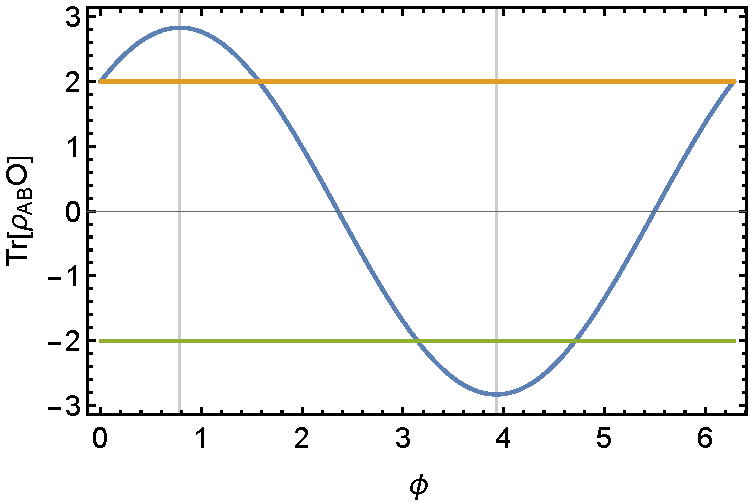
\includegraphics[width=.5\linewidth]{Images/CHSH_plot.pdf}
            \caption{Valor medio del observable CHSH $O$.}
            \label{fig:II_2_c}
        \end{figure}
        
        
        \item Para un sistema de dos qubits, sabemos que
        \[ \rho_{AB}^{t_B} \geq 0 \iff \rho_{AB} \text{ es separable}. \]
        Por lo tanto, para que el estado $\rho$ sea entrelazado, los autovalores de su matriz traspuesta parcial deberán ser negativos.
        En particular para un sistema de dos qubits, donde la matriz densidad se encuentra descrita por
        \begin{align}
            \rho_{AB} = \begin{pmatrix} \mqty{\xmat*{\rho}{4}{4}} \end{pmatrix} \implies \rho^{t_B}_{AB} &=
            \begin{pmatrix}
                \begin{pmatrix} \rho_{11} & \rho_{12} \\ \rho_{21} & \rho_{22} \end{pmatrix}^t & \begin{pmatrix} \rho_{13} & \rho_{14} \\ \rho_{23} & \rho_{24} \end{pmatrix}^t \\
                \begin{pmatrix} \rho_{31} & \rho_{32} \\ \rho_{41} & \rho_{42} \end{pmatrix}^t & \begin{pmatrix} \rho_{33} & \rho_{34} \\ \rho_{43} & \rho_{44} \end{pmatrix}^t \\
            \end{pmatrix} \\
            &=
            \begin{pmatrix}
                \rho_{11} & \rho_{21} & \rho_{13} & \rho_{23} \\
                \rho_{12} & \rho_{22} & \rho_{14} & \rho_{24} \\
                \rho_{31} & \rho_{41} & \rho_{33} & \rho_{43} \\
                \rho_{32} & \rho_{42} & \rho_{34} & \rho_{33} \\
            \end{pmatrix}.
        \end{align}
        
        Por lo tanto, para el caso particular que estamos estudiando,
        \[
            \rho^{t_B}_{AB} =
            \begin{pmatrix}
                \frac{1-x}{4} & 0 & 0 & -\frac{x}{2} \\
                0 & \frac{1-x}{4} + \frac{x}{2} & 0 & 0 \\
                0 & 0 & \frac{1-x}{4} + \frac{x}{2} & 0 \\
                -\frac{x}{2} & 0 & 0 & \frac{1-x}{4}
            \end{pmatrix}.
        \]
        Esta nueva matriz tendrá ahora autovalores
        \[ \lambda_1 = \frac{1 - 3x}{4} < 0 \implies x > \frac{1}{3}, \]
        y
        \[ \lambda_2 = \lambda_3 = \lambda_4 = \frac{1+x}{4} < 0 \implies x < -1. \]
        El segundo caso no corresponde a un estado físico del sistema, por lo que nos reducimos a considerar solo $\lambda_1$. Luego, considerando también que $x \leq 1$, entonces para que el sistema presente entrelazamiento, $x \in \left( \left. \inv{3}, 1 \right] \right.$.
        
        
        \item Para $x \in \left( \left. \inv{3}, 1 \right] \right.$, donde el sistema presentará entrelazamiento, el único autovalor negativo de la matriz $\rho^{t_B}_{AB}$ será $\lambda_1 = (1-3x)/4$, como fue demostrado en el ejercicio anterior. Por lo tanto, $N = -\lambda_1(\rho^{t_B}_{AB}) = (3x - 1)/4$. Para $x \leq 1/3$ no tendremos autovalores negativos de $\rho^{t_B}_{AB}$, por lo que $N = 0$. En general,
        \[
            N(\rho_{AB}) =
            \begin{dcases}
                0, &\text{si } x \in \qty[-\inv{3}, \inv{3}], \\
                \frac{3x - 1}{4}, &\text{si } x \in \left( \left. \inv{3}, 1 \right] \right. .
            \end{dcases}.
        \]
        
        Para un sistema de dos qubits, sabemos que la concurrencia puede ser calculada como 
        \[ C(x) = \max \{ 2 \lambda_{max}(R) - \Tr R, 0 \}, \]
        donde $R$ es la matriz
        \[ R = \qty(\rho_{AB}^{1/2} \ (\sigma_y \otimes \sigma_y) \rho_{AB}^* (\sigma_y \otimes \sigma_y) \ \rho_{AB}^{1/2})^{1/2} = \rho_{AB}. \]
        Finalmente, el entrelazamiento de formación para un sistema de dos qubits estará dado por:
        \[ E(\rho_{AB}) = \sum_{i = 0, 1} p_i \log_2 p_i, \quad \quad p_i = \frac{1 + (-1)^i \sqrt{1 - C^2}}{2}. \]
        
        Las tres magnitudes físicas enunciadas se encuentran representadas gráficamente para este sistema en la figura \ref{fig:II_2_e}.
        
        \begin{figure}[t]
            \centering
            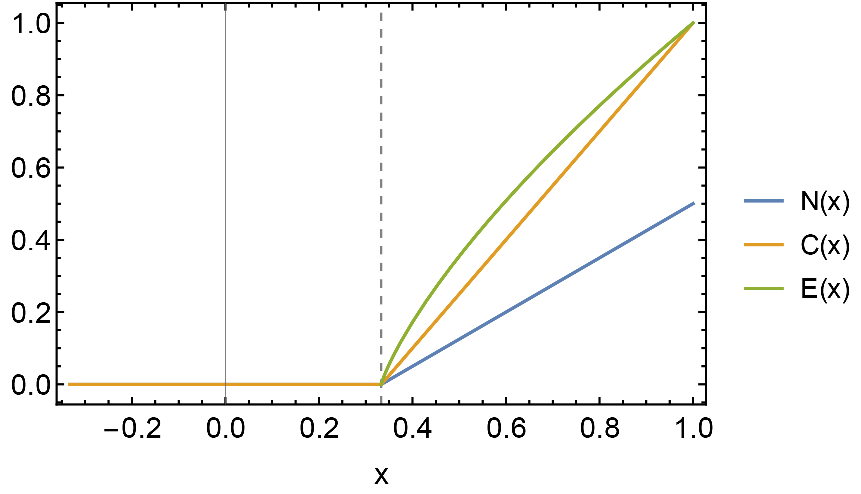
\includegraphics[width=.5\linewidth]{Images/II_2_e-Entanglement.pdf}
            \caption{Negatividad, concurrencia y entrelazamiento de formación para un sistema de dos qubits en el estado $\rho_{AB}$.}
            \label{fig:II_2_e}
        \end{figure}
        
    \end{enumerate}
    
\end{enumerate}
%\nocite{*}
%\printbibliography
\end{document}